\section{Proposed Measurements}


The primary goal of the proposed experiment is to search for a heavy photon (dark photon) in the mass range from 20 MeV to 1000 MeV in at least two settings of beam energy 2.2 GeV and 6.6 GeV. 
HPS  ultimately relies upon the precision measurement of two quantities: the invariant mass of the A$^\prime$ decay products and the position of the decay vertex. By placing a tracking and vertexing detector immediately downstream of the target inside an analyzing magnet, the complete kinematic information required for A$^\prime$ reconstruction can be obtained from a single system, whose proximity to the target naturally maximizes the acceptance of a relatively compact detector and provides excellent momentum and vertexing resolution. A finely segmented, fast electromagnetic calorimeter, just downstream of the tracker,  provides a powerful high rate trigger, identifies electrons, and augments  the electron energy measurement. Behind the ECal a muon system consist of four planes of scintillator hodoscopes sandwiched between iron absorbers will be positioned. The muon system will provide trigger for ($\mu^+\mu^-$) detection and will be used for muon identification. It will extend search for high mass A$^\prime$ in di-muon decay mode where electromagnetic backgrounds are much reduced. Very high rate data acquisition systems, for the tracker, Ecal and muon system, make it possible to trigger and transfer data at $10$s of kHz, and run with negligible dead time.

The HPS experiment also has the potential to discover ``true muonium'', a bound state of a $\mu^+ \mu^-$ pair and to search for non-minimal hidden sector final states.  

\subsection{Search for the heavy photon}
\def \ap {A^\prime}
\def \map {m_{A^\prime}}
\def \thap {\theta_{A^\prime}}
%\subsubsection{Search for a Heavy Photon}
\label{sec:apsignal}

\begin{figure}
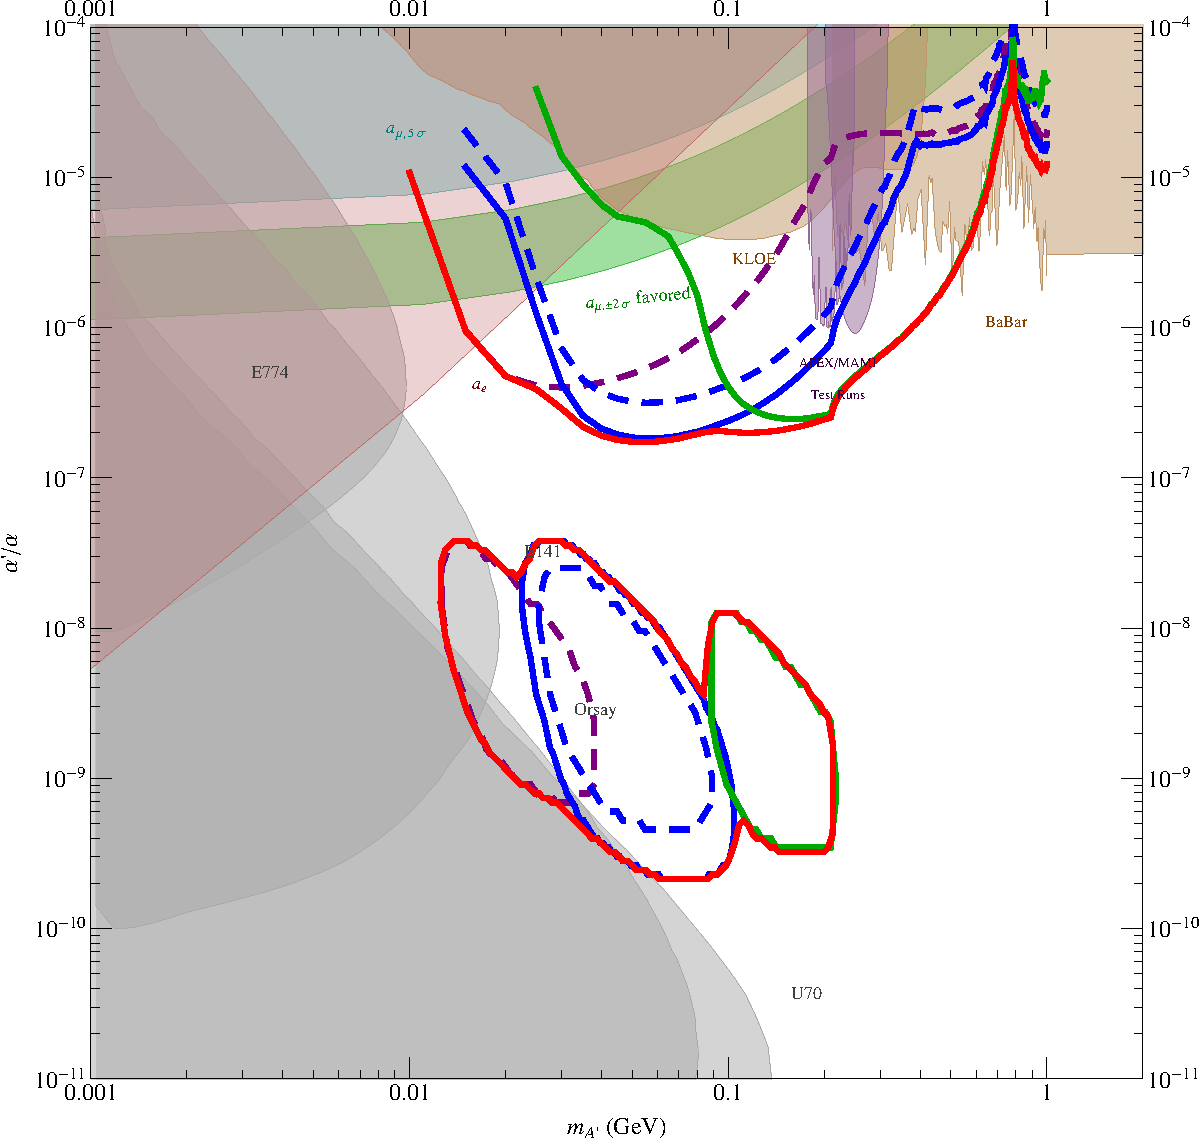
\includegraphics[width=\textwidth]{measurements/HPS-Proposal2014-Reach.pdf}
\caption{Expected mass vs coupling parameter space reach for 2014 running (dashed) and full 2014-2015 running (solid).}
\label{fig:reach}
\end{figure}

HPS plans to execute the experiment in two settings: first, perform a commissioning run with modest physics output, then a longer run at multiple energies to cover as much parameter space as possible. Experimental apparatus will be ready to be commissioned and take physics data in late summer of 2014. The HPS experiment will be ready to use the first physics quality beams available in Hall-B as early as fall of 2014. With assumption that an early running in Hall-B is possible, the run plan for the HPS experiment will be the following: 

\begin{itemize}
\item {\bf Commissioning run in 2014: 2 weeks for setup and hot checkout, 6 weeks on the floor with beam:}
\begin{itemize}
\item 2 weeks of detector commissioning
\item 2 weeks physics run at 2.2 GeV
\item 2 weeks physics run at 1.1 GeV
\end{itemize}
\item{\bf Physics run in 2015, 10 weeks on the floor with beam:}
\begin{itemize}
\item 2 weeks of detector commissioning
\item 4 weeks physics run at 2.2 GeV
\item 4 weeks physics run at 6.6 GeV
\end{itemize}
\end{itemize}

The expected reach with proposed above run plan is shown in Figure \ref{fig:reach}. The reach in mass-coupling parameter space is calculated using the simulated detector response as shown in Section \ref{sec:performance}.  The plot shows two distinct regions,  one at larger coupling corresponding to a purely bump-hunt region and another at lower coupling where the vertex of the $\ap$ decay is displaced.  


\begin{figure}
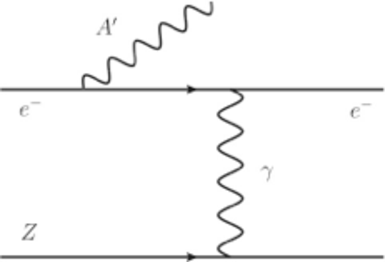
\includegraphics[scale=1]{measurements/Aprime-diagram.pdf}
\caption{Diagram of  $\ap$ production by bremsstrahlung off of an incoming electron scattering with an atomic nucleus.}
\label{fig:apdiagram}
\end{figure}

$\ap$ particles are generated in electron collisions on a fixed target by a process analogous to ordinary photon bremsstrahlung, see Figure \ref{fig:apdiagram}.  The rate and kinematics of $\ap$ radiation differ from massless bremsstrahlung in several important ways:
\begin{itemize}
\item  {\bf Rate}: The total $\ap$ production rate is controlled by $\alpha^3\epsilon^2 / m_{\ap}^2$.  
 Therefore, it is suppressed relative to photon bremsstrahlung by $\sim \epsilon^2 m_e^2/m_{\ap}^2$.  Additional suppression from small $\tilde{\chi}$  occurs for large $m_{\ap}$  or small $E_0$.
\item {\bf Angle}:  $\ap$ emission is dominated at angles$\theta_{\ap}$ such that $U(x,\theta_{\ap}\lesssim 2 U(x,0)$ (beyond this point, wide-angle emission falls as $\theta_{\ap}^4$).  For near it's median value, the cutoff emission angle is
\begin{equation}
\theta_{\ap,max}\sim max\left(\frac{\sqrt{\map m_e}}{E_0},\left(\map/E_0\right)^{3/2}\right),
\end{equation}
which is parametrically smaller than the opening angle of the $\ap$ decay product, $\sim  \map/E_0$.  Although this opening angle is small, the backgrounds mimicking the signal dominate at even smaller angles.
\item {\bf Energy}:  $\ap$ bremsstrahlung is sharply peaked at $\approx 1$, where $U(x,0)$ is minimized.  When an $\ap$ is produced, it carries nearly the entire beam energy.  In fact, the median value of (1-x) is $\sim {\rm max}\left(\frac{m_e}{\map},\frac{\map}{E_0}\right)$.  
\item{\bf Lifetime} For the ranges of $\epsilon$ and $\map$ probed by this experiment, the mean decay length $l_0$ of the $\ap$ can be prompt or as large as tens of centimeters. All of the background decays promptly at the target.  
\end{itemize}
The  latter three properties are quite important in resolving signal events from the main backgrounds, as discussed
below.   More details of $\ap$ production and decay are given in Appendix \ref{app:ProdAndDecay}.

The irreducible background rates are given by the diagrams shown in Figure \ref{fig:radbhdiagram}. These trident events can be usefully separated into 'radiative' diagrams (Figure \ref{fig:radbhdiagram} (a)), and 'Bethe-Heitler' diagrams (Figure \ref{fig:radbhdiagram} (b)), that are separately gauge-invariant.  These QED tridents dominate the final event sample, so we consider their properties in some detail here.

\begin{figure}
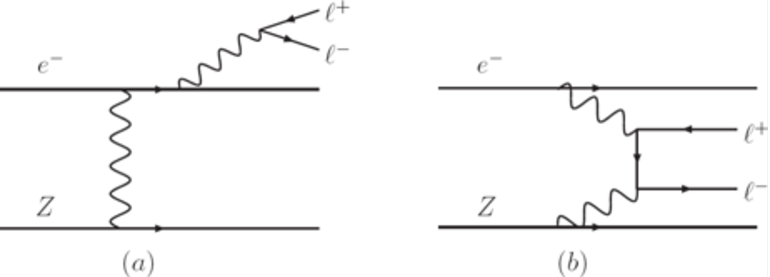
\includegraphics[scale=1]{measurements/rad-bh-diagrams.pdf}
\caption{Sample diagrams of (left) radiative trident ($\gamma^*$) and (right) Bethe-Heitler trident reactions that comprise the primary background to the $\ap\rarr l^+l^-$  search.}
\label{fig:radbhdiagram}
\end{figure}

The contribution from the radiative diagrams (Figure \ref{fig:radbhdiagram} (a)) alone is also useful as a guide to the behavior of $\ap$ signals at various masses. Indeed, the kinematics of the A' signal events is identical to the distribution of radiative trident events restricted in an invariant mass window near the A' mass. Moreover, the rate of the A' signal is simply related to the radiative trident cross-section within the spectrometer acceptance and a mass window of width $\delta m$ by \cite{4}
\begin{equation}
\frac{d\sigma\left(e^- Z \rarr e^- Z(\ap\rarr l^+l^-)\right)}{d\sigma\left(e^- Z \rarr e^- Z(\gamma^*\rarr l^+l^-)\right)}=\frac{3\pi\epsilon^2}{2 N_{eff}\alpha}\frac{\map}{\delta m}
\end{equation}
This exact analytic formula was also checked with a MC simulation of both the $\ap$ signal and the radiative trident background restricted to a small mass window $\delta m$, and we find nearly perfect agreement. Thus, the radiative subsample can be used to analyze the signal, which simplifies the analysis considerably.

 Although the Bethe-Heitler process has a much larger total cross-section than either the signal or the radiative trident background, it can be significantly reduced by exploiting its very different kinematics. In particular, the $\ap$ carries most of the beam energy (see discussion in Section \ref{sec:apsignal}), while the recoiling electron is very soft and scatters to a wide angle. In contrast, the Bethe-Heitler process is not enhanced at high pair energies. Moreover, Bethe-Heitler processes have a forward singularity that strongly favors asymmetric configurations with one energetic, forward electron or positron and the other constituent of the pair much softer.
These properties are discussed further in the Appendix of [4], and illustrated in Figure \ref{fig:tridentkinematics}.

\begin{figure}
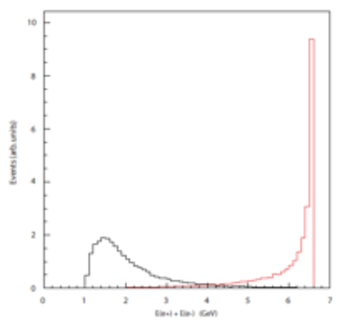
\includegraphics[scale=1]{measurements/rad-bh-energy.pdf}
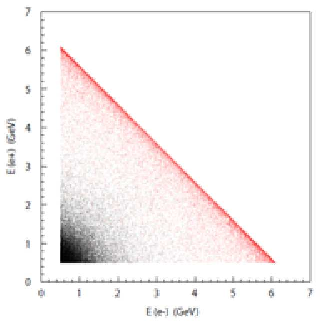
\includegraphics[scale=1]{measurements/E1vsE2.pdf}
\caption{ Left: The distribution of Bethe-Heitler background events (black) and $\ap$ signal events (red) as a function of the sum of the electron and positron energy. Note that the signal is peaked at high energies, while the background is peaked at much lower energies. Right: The distribution of the positron versus electron energy for Bethe-Heitler background events (black dots) and A’ signal events (red dots). Note that in both plots neither the signal nor background events have been normalized to the correct number. In reality, the number of background events is much larger than the number of signal events. Also, note that the electron energy here refers to the energy of the electron produced in the reaction, not the recoiling beam electron.}
\label{fig:tridentkinematics}
\end{figure}



\subsection{Search for true muonium}

The proposed HPS experiment has the potential to discover ``true muonium'', a bound state of a
$\mu^+ \mu^-$ pair, denoted here by $(\mu^+ \mu^-)$. 
We expect that HPS will discover the 1S, 2S, and 2P true muonium bound states with its proposed run plan. 
The detection of these states should demonstrate the capability of the HPS experiment 
to identify rare separated vertex decays, and will provide a natural calibration 
tool for improving searches for heavy photons. Details of the production and detection of true muonium using HPS detector can be found in \cite{HPS_PROP_UPD}. 
The $(\mu^+ \mu^-)$ atom is hydrogen-like, and so has a set of excited states characterized by a principal quantum number n. 
The binding energy of these states is E = $-1407$ eV/n$^2$. The $(\mu^+ \mu^-)$ ``atom'' can be produced by an electron beam incident on a target such 
as tungsten \cite{Holvik:1986ty,ArteagaRomero:2000yh}. 

With the existing proposal, HPS will search for true muonium
just as it does for heavy photons with separated vertices, requiring a vertex cut at about 1.5 cm to reject almost all
QED background events, then searching for a resonance at 2 m$_{\mu}$. An additional cut 
on the total energy of the $e^+e^-$ pair of $E_{e^-}+E_{e^+}> 0.8 \ E_{beam}$ will also be required
for triggering. 

Based on \cite{toAppear}, the total production yield for 1S, 2S, and 2P (including secondary production)
leaving a target of thickness $t_b$(or larger) and satisfying the above requirements is,
\begin{equation}
N_{(\mu^+ \mu^-)} = 200 \left( \frac{I}{450 \ nA} \right) \left( \frac{t}{1 \ month} \right)
\end{equation}
%
where a beam energy E$_{beam} = 6.6$ GeV, and the nominal conditions
of 450 nA beam current for 1 months ($\sim 2.6 \times 10^6$ s) on a single foil has been assumed.
The vertices near the cut of $1.5$ cm will be dominated by the 1S state, while 
a tail of vertices extending out beyond a few cm is dominated by 2S and 2P. 

Accounting for all the efficiencies associated with a separated vertex search, we would expect to see about 20--335 true muonium events 
(we caution that the acceptance parameterization here is uncertain at the 50\% level).
The HPS experiment should be able to identify enough events to claim a discovery, and in addition, should be able to measure the mass of true muonium.  There are certainly other properties of true muonium that would be interesting to measure.  A measurement of the lifetimes would be interesting, as the lifetimes are sensitive to physics that couples to leptonic currents.  With enough statistics, it should be possible to perform a measurement of the lifetimes of the 1S, 2S, and 2P states; work is ongoing to investigate this possibility.  

\subsection{Other searches for hidden sector particles}


While the primary motivation for the conception of the HPS experiment is a search for $\ap$ decaying to lepton pairs, following Arkani-Hamed et al, we should make sure that HPS is sensitive to other kinds of Hidden Valley (HV) scenarios. As Strassler and Zurek pointed out, HV provide plethora of natural ways to explain the nature of the Dark Matter. The recent discovery of a boson that seems to have the properties of the Higgs boson of the Standard model also brings an old problem to the fore – why is the Higgs mass is so light compare to the Planck scale? Searches for supersymmetric partners and other particles with strong and/or weak charges at the energy frontier so far came out negative, pushing the range of allowed masses for such particles higher and higher. HPS will be the first in hopefully a series of experiments that complements the energy frontier by looking for light particles that couple to the SM particles through new, very weak forces. Just as exploring the energy frontier at the LHC one should be ready for unexpected, so should we be exploring the coupling frontier at the HPS.

In a general HV scenario, the new fermions may be lighter then the $\ap$ and have their own QCD-like forces forming hidden mesons and baryons some of which could be constituents of Dark Matter. Some of such mesons would decay into SM fermion pairs – either democratically or with mass-dependent branchings. 
\begin{figure}
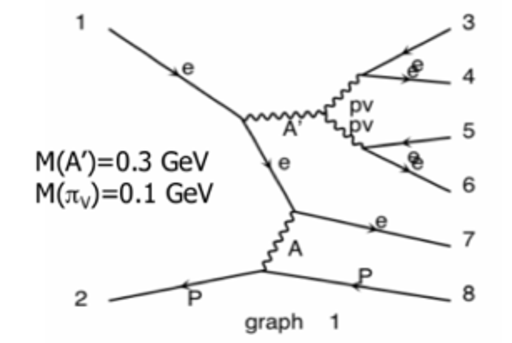
\includegraphics[scale=1]{measurements/multilepton-diagram.pdf}
\caption{Sample diagram of a non-Abelian hidden sector interaction.}
\label{fig:mldiagram}
\end{figure}
One possible  case is where the $\ap$ decays into a pair of dark mesons ($\pi_v$), which in turn promptly decay into electron pairs (see Fig \ref{fig:mldiagram}).  The high multiplicity of the typical final states makes an exclusive search for events such as these  difficult to trigger upon, it also reduces the background by a large amount as well as providing a number of possible invariant mass bumps to search for and find.  Simulation is ongoing towards estimating the reach HPS has for these states.  


%
%
%In the simulation, we took $\ap$ and $\pi_v$ masses to be 0.3 and 0.1 GeV respectively. We generated 25,000 events at 2.2 GeV incoming beam and put them through the full simulation and reconstruction.
%
%We found that the probability of having all four electrons in the detector acceptance is fairly small. Only XXX events had 4 or more reconstructed tracks and of those more then half had (fake, misreconstructed, other background) tracks. Once we required two $\pi_v$ candidates with consistent masses ($\Delta M<0.025$ GeV) the $\ap$ signal is clearly visible in the two-dimensional plane of average $\pi_v$ mass and $\ap$ mass (see Fig \ref{fig:mlinvmass})     
%The resulting signal efficiency is $50/25000 \sim 2\times 10^{-3}$.
%
%
%\begin{figure}
%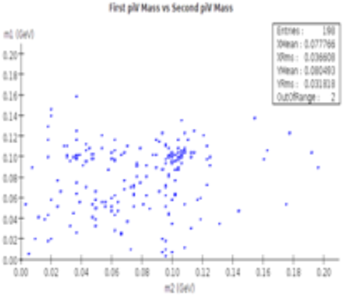
\includegraphics[scale=1]{measurements/ML-m1vsm2pdf.pdf}
%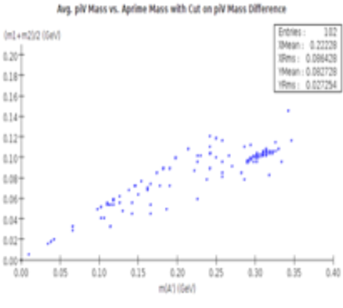
\includegraphics[scale=1]{measurements/ML-mAvsmAvgf.pdf}
%\caption{Left:  Invariant masses of the two reconstructed $\pi_v$ candidates.  Right:  The 4-lepton invariant mass verses the average  $\pi_v$ candidate mass.}
%\label{fig:mlinvmass}
%\end{figure}
% 
%	In an effort to enhance the signal efficiency we tried to take advantage of the fact that $\ap$ is produced with very little transverse momentum. Therefore, in the events with just three reconstructed electrons, we assume that the fourth electron is out of acceptance, and its transverse momentum is equal to minus the sum of the transverse momenta of the three reconstructed electrons. The longitudinal momentum of the fourth electron is then given, with two-fold ambiguity, by requiring the $\pi_v$ candidate it makes to have the same mass as the fully reconstructed $\pi_v$. We resolve the ambiguity by picking the solution with the largest longitudinal momentum, as long as the total $\ap$ energy does not exceed the incoming beam energy. Thus reconstructed $\pi_v$ and $\ap$ mass distributions are shown in Fig \ref{fig:mlreciolmass} (each event can give up to two entries since there are two possible reconstructed $\pi_v$ hypotheses). The $\ap$ mass resolution is 0.07 GeV, and the signal efficiency is around 3\%.
%
%
%
%\begin{figure}
%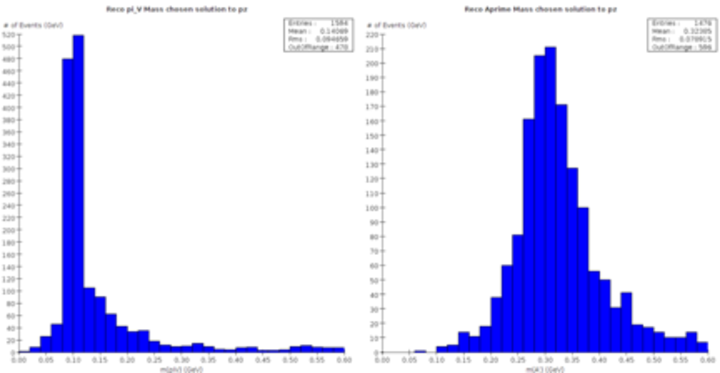
\includegraphics[scale=1]{measurements/ML-recoilMass.pdf}
%\caption{Left:  The $\pi_v$ candidate recoill mass.  Right:  The $\ap$ candidate recoil mass.}
%\label{fig:mlreciolmass}
%\end{figure}
%
%	We estimated the background using the same simulated QED trident sample as for the baseline $\ap$ search… (results of that study here)
